\documentclass[a4paper,
fontsize=11pt,
%headings=small,
oneside,
numbers=noperiodatend,
parskip=half-,
bibliography=totoc,
final
]{scrartcl}

\usepackage[babel]{csquotes}
\usepackage{synttree}
\usepackage{graphicx}
\setkeys{Gin}{width=.4\textwidth} %default pics size

\graphicspath{{./plots/}}
\usepackage[ngerman]{babel}
\usepackage[T1]{fontenc}
%\usepackage{amsmath}
\usepackage[utf8x]{inputenc}
\usepackage [hyphens]{url}
\usepackage{booktabs} 
\usepackage[left=2.4cm,right=2.4cm,top=2.3cm,bottom=2cm,includeheadfoot]{geometry}
\usepackage{eurosym}
\usepackage{multirow}
\usepackage[ngerman]{varioref}
\setcapindent{1em}
\renewcommand{\labelitemi}{--}
\usepackage{paralist}
\usepackage{pdfpages}
\usepackage{lscape}
\usepackage{float}
\usepackage{acronym}
\usepackage{eurosym}
\usepackage{longtable,lscape}
\usepackage{mathpazo}
\usepackage[normalem]{ulem} %emphasize weiterhin kursiv
\usepackage[flushmargin,ragged]{footmisc} % left align footnote
\usepackage{ccicons} 
\setcapindent{0pt} % no indentation in captions

%%%% fancy LIBREAS URL color 
\usepackage{xcolor}
\definecolor{libreas}{RGB}{112,0,0}

\usepackage{listings}

\urlstyle{same}  % don't use monospace font for urls

\usepackage[fleqn]{amsmath}

%adjust fontsize for part

\usepackage{sectsty}
\partfont{\large}

%Das BibTeX-Zeichen mit \BibTeX setzen:
\def\symbol#1{\char #1\relax}
\def\bsl{{\tt\symbol{'134}}}
\def\BibTeX{{\rm B\kern-.05em{\sc i\kern-.025em b}\kern-.08em
    T\kern-.1667em\lower.7ex\hbox{E}\kern-.125emX}}

\usepackage{fancyhdr}
\fancyhf{}
\pagestyle{fancyplain}
\fancyhead[R]{\thepage}

% make sure bookmarks are created eventough sections are not numbered!
% uncommend if sections are numbered (bookmarks created by default)
\makeatletter
\renewcommand\@seccntformat[1]{}
\makeatother

% typo setup
\clubpenalty = 10000
\widowpenalty = 10000
\displaywidowpenalty = 10000

\usepackage{hyperxmp}
\usepackage[colorlinks, linkcolor=black,citecolor=black, urlcolor=libreas,
breaklinks= true,bookmarks=true,bookmarksopen=true]{hyperref}
\usepackage{breakurl}

%meta
%meta

\fancyhead[L]{Redaktion LIBREAS\\ %author
LIBREAS. Library Ideas, 41 (2022). % journal, issue, volume.
\href{https://doi.org/10.18452/24796}{\color{black}https://doi.org/10.18452/24796}
{}} % doi 
\fancyhead[R]{\thepage} %page number
\fancyfoot[L] {\ccLogo \ccAttribution\ \href{https://creativecommons.org/licenses/by/4.0/}{\color{black}Creative Commons BY 4.0}}  %licence
\fancyfoot[R] {ISSN: 1860-7950}

\title{\LARGE{Editorial \#41: Big Scholarly Data}}% title
\author{Redaktion LIBREAS} % author

\setcounter{page}{1}

\hypersetup{%
      pdftitle={Editorial \#41: Big Scholarly Data},
      pdfauthor={Redaktion LIBREAS},
      pdfcopyright={CC BY 4.0 International},
      pdfsubject={LIBREAS. Library Ideas, 41 (2022)},
      pdfkeywords={Open Access, Big Scholarly Data},
      pdflicenseurl={https://creativecommons.org/licenses/by/4.0/},
      pdfcontacturl={https://libreas.eu},
      baseurl={},
      pdflang={de},
      pdfmetalang={de},
      pdfdoi={10.18452/24796},
      pdfurl={https://doi.org/10.18452/24796}
     }



\date{}
\begin{document}

\maketitle
\thispagestyle{fancyplain} 

%abstracts

%body
Diese Ausgabe ist Zeugnis einer Schwerpunktverlagerung -- und zwar vom
Konkreten zum Allgemeinen und zurück zu einem anderen Konkreten. War der
Ausgangspunkt unseres Call for Paper noch der Verlust von Microsoft
Academic Services und damit das Einfrieren des Microsoft Academic Graph
(MAG), einer großen und frei verfügbaren Datensammlung über
wissenschaftliche Literatur, so scheinen mittlerweile eher Fragen nach
dem Umfang und der Vielfalt der Landschaft von Big Scholarly Data von
hoher Relevanz für Bibliotheken und Informationseinrichtungen.
Insbesondere das Ende 2021 öffentlichkeitswirksam gestartete OpenAlex,
vom Anspruch her eine Art Weltkatalog des wissenschaftlichen
Publikationsaufkommens,\footnote{Singh Chawla, D. (2022). Massive open
  index of scholarly papers launches. Nature.
  \url{https://doi.org/10.1038/d41586-022-00138-y}} wird in Forschung
und Praxis als offene Alternative zu den kommerziellen
Bibliometriedatenbanken wie dem Web of Science, Scopus oder Dimensions
erörtert.

Zugleich schlägt sich etwa im Informationspapier \enquote{Datentracking
in der Wissenschaft} des Ausschusses für Wissenschaftliche Bibliotheken
und Informationssysteme der Deutschen Forschungsgemeinschaft\footnote{Ausschuss
  für Wissenschaftliche Bibliotheken und Informationssysteme der
  Deutschen Forschungsgemeinschaft (2021). Datentracking in der
  Wissenschaft: Aggregation und Verwendung bzw. Verkauf von
  Nutzungsdaten durch Wissenschaftsverlage.
  \url{https://www.dfg.de/download/pdf/foerderung/programme/lis/datentracking_papier_de.pdf}}
ein gestiegenes Bewusstsein über negative Folgen des Wandels der
Geschäftsmodelle wissenschaftlicher Verlage in Richtung Data Analytics
für Wissenschaft und Bibliotheken nieder. Paradoxerweise würde gerade
das ursprünglich als Gegenmodell zur übermäßigen Kommodifizierung der
Wissenschaft angedachte Konzept des Open Access heute zu neuen
verlagsspezifischen Plattformlösungen führen. Großverlage bereiten Daten
über wissenschaftliche Informationsprozesse auf und bieten diese
wissenschaftlichen Einrichtungen für die Unterstützung komplexer
Entscheidungsfindungen an, etwa im Kontext der Anbahnung und Evaluation
von Open-Access-Transformationsverträgen.\footnote{Scholl, D. (2021).
  Datentracking: Die schöne neue Welt der Wissenschaftsverlag. Wikimedia
  Deutschland.
  \url{https://blog.wikimedia.de/2021/12/07/datentracking-die-schoene-neue-welt-der-wissenschaftsverlage/}}

Dahingegen glauben wir, dass der souveräne, also anbieterunabhängige
Umgang mit Big Scholarly Data in der bibliothekarischen Berufspraxis ein
Schlüssel ist, um diesen Trend der Kommodifizierung von Daten über
wissenschaftliche Publikationen zu begegnen. Wir freuen uns daher, in
der Ausgabe \#41 vielfältige Anwendungsbeispiele von Big Scholarly Data
für die Beantwortung von bibliothekarischen Informationsbedürfnissen
versammeln zu dürfen.

\begin{figure}
\centering
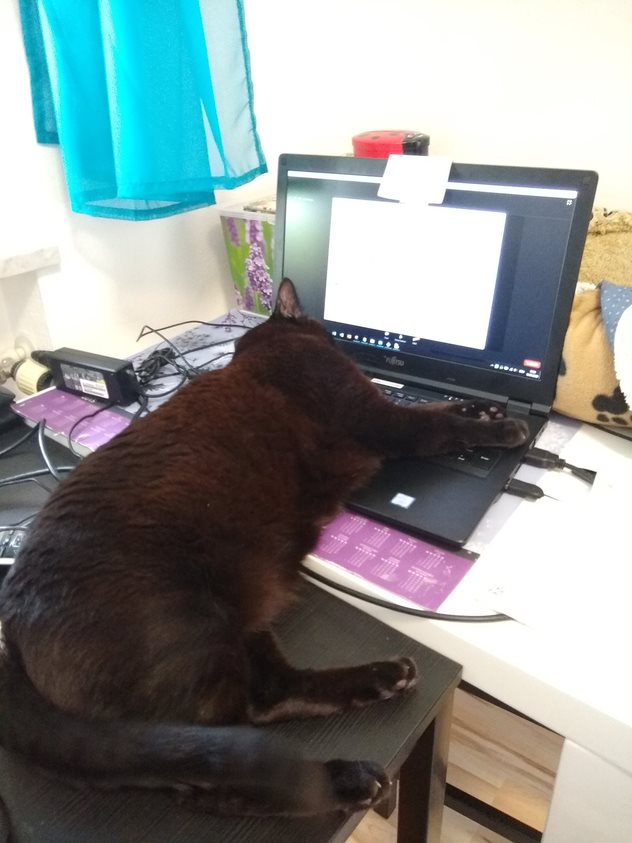
\includegraphics{image.png}
\caption{Redaktionsorte XX: Arbeitstreffen online.}
\end{figure}

In ihrem Werkstatbericht stellen Franziska Stanzel, Irene Barbers,
Philipp Pollack und Barbara Lindstrot von der Bibliothek des
Forschungszentrums Jülich ihre Arbeit mit kommerziellen als auch offenen
Datensätzen im Kontext des Open Access Monitors vor. Sie gehen dabei
insbesondere auf ihre Normierungsaufwände ein, die entstehen, wenn
unterschiedliche Datenquellen miteinander kombiniert werden.

Die Beraterin und Projektmanagerin Anne Christensen erläutert die Frage
nach Gemeinsamkeiten und Unterschieden zwischen akademischen
Suchmaschinen und den in Bibliotheken eingesetzten Discovery-Systemen.
Sie sieht sowohl bezogen auf die Usability als auch der Öffnung der
Datenbestände ein großes Potenzial für Discovery-Systeme, damit sie
stärker als bisher mit ihren zugrunde liegenden Erschließungsverfahren
als Suchraum für wissenschaftliche Literatur sowie als Grundlage für
Datenanalysen wahrgenommen werden.

Philipp Zumstein, Universitätsbibliothek Mannheim, nutzt offene Daten,
um die Publikationspraxis des Mega-Journals Academia Letters zu
beschreiben. Insbesondere die Vernetzung mit dem sozialen Netzwerk
Academia und ein Einreichungs- und Begutachtungsworkflow, der auf kurze
Fristen setzt, sind mögliche Erklärungen für die gestiegene Anzahl an
Artikeln, die in den letzten Monaten im Journal veröffentlicht wurden.
Er beleuchtet zudem Aspekte der (fehlenden) Qualitätssicherung und
Transparenz des Publikationsservice.

Nick Haupka, Najko Jahn und Anne Hobert von der SUB Göttingen
illustrieren abschließend, wie sie dank Cloud-Computing-Umgebung auch
ohne eigene Datenbank- und Serveradministration Analysen großer
Datenmengen bewerkstelligen. Dabei fokussieren sie auf die Datenquellen
Unpaywall, Crossref und OpenAlex, die etwa für die Beantwortung von
Fragestellungen im Kontext des hybriden Open Access genutzt werden.

Neben diesen Schwerpunktbeiträgen untersucht der
Bibliothekswissenschaftler Karsten Schuldt die Einführung von Minitel
und Btx an Bibliotheken in den 1980er Jahren als ein zeithistorisches
Beispiel, wie Bibliotheken neue Technologien aufgriffen. Und
selbstverständlich fasst auch in dieser Ausgabe die Kolumne DLDL in der
Tradition einer Referatezeitschrift fachliche Beiträge zusammen. Obwohl
man heute vielleicht noch überzeugender wirken könnte, wenn man von
einem Small-Scholarly-Data-Graphen spricht. Gern weisen wir zudem darauf
hin, dass die bibliografischen Daten der in DLDL besprochenen Beiträge
nun in einer öffentlich zugänglichen Zotero-Gruppe zu finden sind:
\url{https://www.zotero.org/groups/4620604/libreas_dldl/library}

Viel Vergnügen und Anregung wünscht die LIBREAS Redaktion!

(Berlin, Hannover, Göttingen, Lausanne, München, Potsdam)

%autor

\end{document}
